\documentclass[pdf, fleqn, compress]{beamer}
\usepackage{york-beamer-template}
\usepackage{tikz-cd}

\graphicspath{{./fig/}}

%	Font style for emphasis
\newcommand{\mathsterm}[1]{{\itshape\color{dark-teal!80}#1}}

\setlist[itemize,1]{itemsep=1em, leftmargin=0em}
\setitemize{label=\usebeamerfont*{itemize item}%
  \usebeamercolor[dark-teal!50!ebor]{itemize item}
  \usebeamertemplate{itemize item}}

\title[Short Title]{Long Title}
\author[J. Bloggs]{Jonathon Johnson Bloggs III}
\institute{Institution (Probably York)}
\date{\today}

\begin{document}

%	nonavigation environment defined in york-beamer-template.sty
\begin{nonavigation}
%-------------------------------------------------------------------
%   Begin Frontmatter (Frames here have no head/foot and no logo)
%-------------------------------------------------------------------

\begin{frame}
    \titlepage
\end{frame}

%-------------------------------------------------------------------
%   End Frontmatter
%-------------------------------------------------------------------
\end{nonavigation}

%-------------------------------------------------------------------
%   NOTE: Top bar appears as in nonavigation environment
%		  if no sections are defined
%-------------------------------------------------------------------

\section{Section 1}

\begin{frame}{Frame 1}
	What is a Frame
	\begin{itemize}
		\item A slide in beamer
		\pause
		\item That may contain pauses
		\begin{itemize}
			\item Lists may also have lists embedded within them
		\end{itemize}
	\end{itemize}
\end{frame}

\section{Section 2}

\begin{frame}{Frame}
	\begin{itemize}
		\item Frames may also have equations
		\begin{equation}
			E^2 = p^2 c^2 + m^2 c^4
		\end{equation}
		\item We can also do citations \cite{knuth1986computers}.
	\end{itemize}
\end{frame}

\begin{frame}[fragile]{Tikz}
	\begin{itemize}
		\item	Just a friendly reminder that frames containing Tikz diagrams need the \texttt{[fragile]} tag
				\begin{equation}
					\begin{tikzcd}
						&
						T(V)
							\ar[d, dashed, "\exists ! \phi"]
						\\
						V
							\ar[ur, hookrightarrow, "\iota"]
							\ar[r, swap, "\forall \rho"]
						&
						W		
					\end{tikzcd}
				\end{equation}
	\end{itemize}
\end{frame}

\begin{frame}{It Figures}
	\begin{figure}
		\centering
			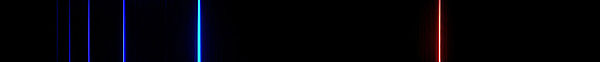
\includegraphics[width=\linewidth]{BalmerVisible}
		\caption{Images placed in the \texttt{./fig} folder can be included without specifying a path or file extension.}
	\end{figure}
\end{frame}

\begin{frame}{Environments}
	\begin{definition}
		This is a \mathsterm{definition}.
	\end{definition}

	\begin{prop}
		This is a \mathsterm{proposition}.
	\end{prop}

	\begin{theorem}
		This is a \mathsterm{theorem}.
	\end{theorem}

	\begin{corollary}
		This is a \mathsterm{corollary}
	\end{corollary}
\end{frame}
\begin{nonavigation}
\appendix

\begin{frame}{References}
	\fontsize{8pt}{7.2}\selectfont
	\bibliographystyle{alpha}
	\bibliography{biblio}
\end{frame}

\end{nonavigation}

\end{document}
